{\chapter{Evaluation: Queries}
\label{chap:Eval_6}


In (\ref{chap:Eval_5}), we presented the first part of the evaluation results for the experiments we conducted on the graph structures in order to evaluate their performance. With the first part of the evaluation results, we managed to give answers for the evaluation questions (1, 2, and 3) which we have stated in (\ref{sec:EvalQuests}) concerning the scalability, batch loading, and parallel loading of the graph structures.

In this chapter, we present the second and last part of the evaluation results for the experiments we conducted on the graph structures. The evaluation experiments which we present in this chapter are aiming to evaluate the performance of the graph structures in query execution. All the experiments we conducted are using the evaluation dataset which we presented in (\ref{sec:dataset}). We aim to exploit the evaluation results which we present in this chapter in order to give answers for the evaluation question number (4) which we have stated in (\ref{sec:EvalQuests}) concerning the effect of graph structure choice on the query response time. This chapter is consisted of the following sections:

\begin{itemize}  

\item \textbf{Evaluation: Query \#1:}\\
In section (\ref{sec:eval-qry1}), we present the evaluation results concerning the performance of the graph data structures to execute Query \#1.

\item \textbf{Evaluation: Query \#2:}\\
In section (\ref{sec:eval-qry2}), we present the evaluation results concerning the performance of the graph data structures to execute Query \#2.

\item \textbf{Evaluation: Query \#3:}\\
In section (\ref{sec:eval-qry3}), we present the evaluation results concerning the performance of the graph data structures to execute Query \#3.

\item \textbf{Summary:}\\
Lastly, we provide a summary for what we discussed in the chapter. (\ref{sec:eval-summary_part2})

\end{itemize}



\begin{figure}[H]
\centering
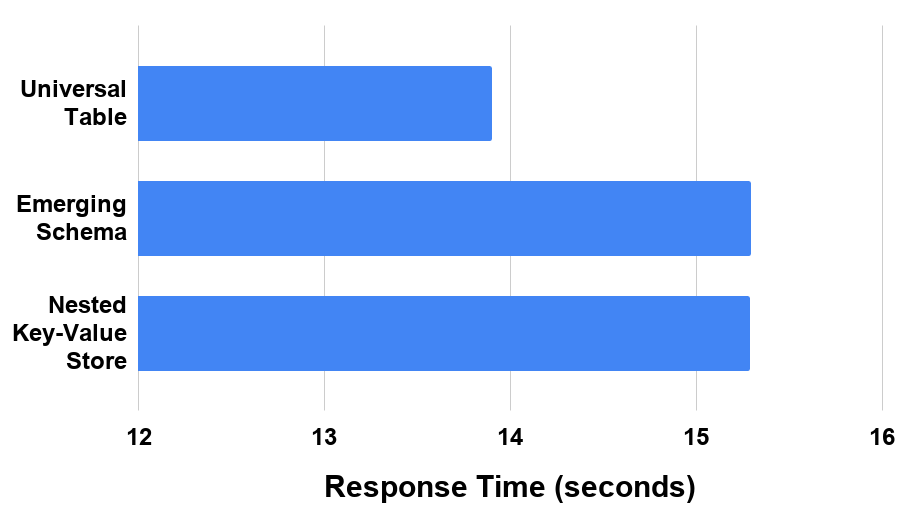
\includegraphics[width=0.7\textwidth]{pics/Query1-Eval.png}
\caption{Response time of Query \#1.}
\label{fig:eval-query1}
\end{figure} 



\section{Evaluation: Query \#1}
\label{sec:eval-qry1}

In this section, we present the evaluation results for the query response time of \mbox{Query \#1} when executed on the data stored in the different graph structures. We defined \mbox{Query \#1} in (\ref{subsec:qry1}). \mbox{Query \#1} is an example of a simple pattern-matching query that requires no traversals between the graph elements.


\begin{itemize}

\item \textbf{Experiment Setup:}\\
In this experiment we used the batch data loader to load the evaluation dataset into the graph structures. We fixed the batch size of the loader to (1000). Query \#1 requires only as an input the properties of each vertex, therefore we loaded the evaluation dataset only into the graph properties structures. We loaded the evaluation dataset with scale factor (4) into each graph properties structure and executed the query for twenty times and recorded the query response time of each run. We took the average of the measured figures after removing the most top and least figures. We set the query parameters in this experiment to the following values: (\textit{\$date = "2011-07-21T22:00:00"}).


\item \textbf{Expected Result:}\\
We expect the response time of Query \#1 on universal table to be the lowest and on emerging schema to be the highest.


\item \textbf{Observation:}\\
We observed that universal table has recorded the lowest response time for Query \#1 with only (13.901 seconds). Also, we observed that the nested key-value store came in the second place with a response time of (15.285 seconds) and at the last place came the emerging schema structure with (15.293 seconds) not far from the nested key-value store. In (\ref{fig:eval-query1}), we show a chart depicting Query \#1 response time when executed on the different graph properties structures.

\item \textbf{Conclusion:}\\
To answer question number (4) from the evaluation questions listed in (\ref{sec:EvalQuests}), the evaluation results are showing that the universal table structure has the lowest response time when executing a simple pattern-matching query that requires no traversals between the graph elements. Universal table response time for Query \#1 is less by (9\%) than emerging schema and nested key-value store.

\end{itemize}



\section{Evaluation: Query \#2}
\label{sec:eval-qry2}


In this section, we present the evaluation results for the query response time of \mbox{Query \#2} when executed on the data stored in the different graph structures. We defined \mbox{Query \#2} in (\ref{subsec:qry2}). \mbox{Query \#2} is an example of a complex pattern-matching query that requires traversals between the graph elements in order to fulfill the query requirements.


\begin{itemize}

\item \textbf{Experiment Setup:}\\
In this experiment we used the batch data loader to load the evaluation dataset into the graph structures. We fixed the batch size of the batch loader to (1000). Query \#2 requires as an input both: the properties of each vertex as well as the topology of the graph, therefore we loaded the evaluation dataset into every possible combination of a graph properties structure and a graph topology structure. We loaded the evaluation dataset with scale factor (4). We excluded the adjacency matrix out of this test due to the scalability issue we faced when we tried to load the evaluation dataset into the adjacency matrix \textit{(see \ref{subsec:scalability-topology})}. We loaded the data into each graph structure and executed the query for twenty times and recorded the query response time of each run. We took the average of the measured figures after removing the most top and least figures. We set the query parameters in this experiment to the following values: (\textit{\$date = "2011-07-22T00:00:00", \$lengthThreshold = "20", \$languages = \{"ar"\}}).



\begin{figure}[H]
\centering
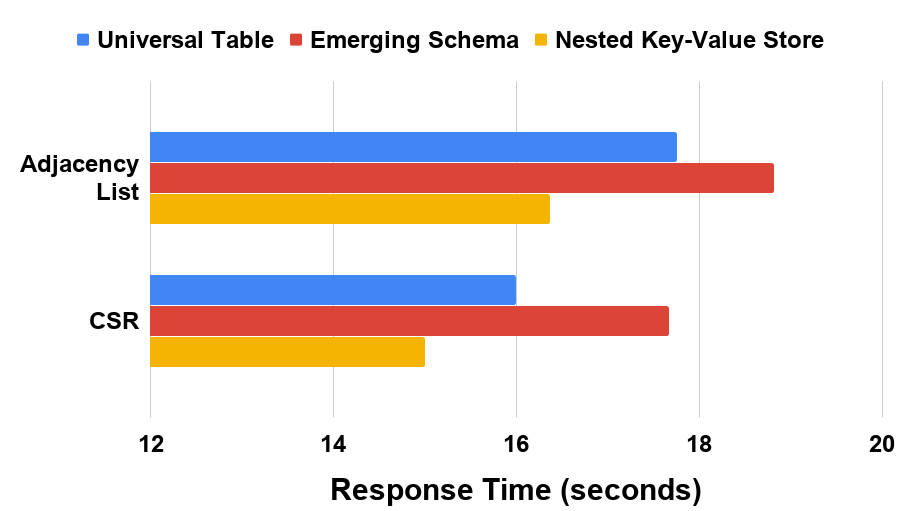
\includegraphics[width=0.7\textwidth]{pics/Query2-Eval.png}
\caption{Response time of Query \#2.}
\label{fig:eval-query2}
\end{figure} 

\item \textbf{Expected Result:}\\
We expect the response time of Query \#2 on the combination of graph structures where the compressed sparse row (CSR) is part of to be lower than the response time of those where the adjacency list is part of. Also, we expect the response time of Query \#2 on the combination of graph structures where the universal table is part of to be lower than the response time of those where the emerging schema or the nested key-value store is part of.

\item \textbf{Observation:}\\
We observed that the combination of compressed sparse row (CSR) along with nested key-value store has recorded the lowest response time for Query \#2 with only (15 seconds). Also, we observed that the combination of adjacency list along with emerging schema has recorded the highest response time (18.819 seconds). 

The combination of graph structures where the nested key-value store is part of has recorded lower response time for Query \#2 than the response time of those where the universal table or the emerging schema is part of. Also, the combination of graph structures where the compressed sparse row (CSR) is part of has recorded lower response time for Query \#2 than the response time of those where the adjacency list is part of. 

In (\ref{fig:eval-query2}), we show a chart depicting Query \#2 response time when executed on the different combinations of graph properties structures and graph topology structures.

\item \textbf{Conclusion:}\\
To answer question number (4) from the evaluation questions listed in (\ref{sec:EvalQuests}), the evaluation results are showing that the combination of compressed sparse row (CSR) along with nested key-value store has the lowest response time when executing a a complex pattern-matching query that requires traversals between the graph elements in order to fulfill the query requirements.

\end{itemize}

\section{Evaluation: Query \#3}
\label{sec:eval-qry3}

In this section, we present the evaluation results for the query response time of \mbox{Query \#3} when executed on the data stored in the different graph structures. We defined \mbox{Query \#3} in (\ref{subsec:qry3}). \mbox{Query \#3} is computing the performing a degree centrality report for the graph topology.
\begin{figure}[H]
\centering
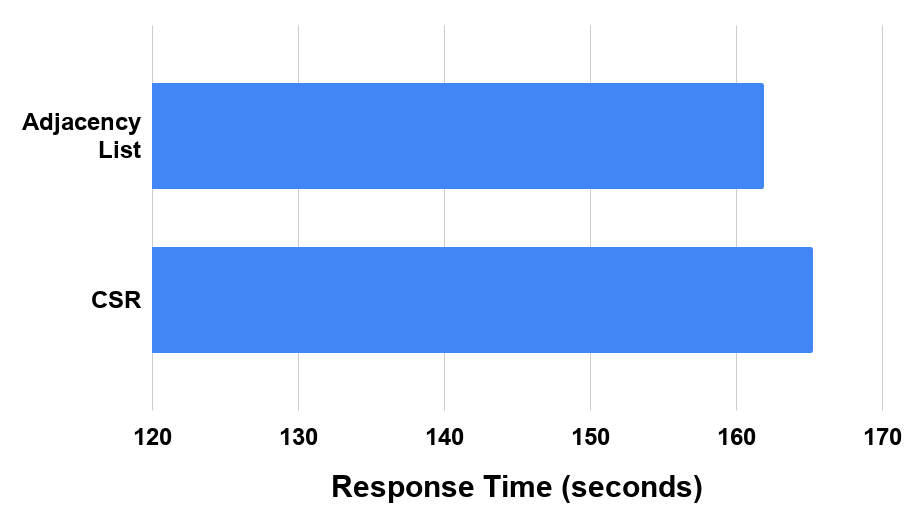
\includegraphics[width=0.7\textwidth]{pics/Query3-Eval.png}
\caption{Response time of Query \#3.}
\label{fig:eval-query3}
\end{figure} 

\begin{itemize}
\item \textbf{Experiment Setup:}\\
In this experiment we used the batch data loader to load the evaluation dataset into the graph structures. We fixed the batch size of the batch loader to (1000). Query \#3 requires only as an input the properties of each vertex, therefore we loaded the evaluation dataset only into the graph topology structures. We loaded the evaluation dataset with scale factor (4). We excluded the adjacency matrix out of this test due to the scalability issue we faced when we tried to load the evaluation dataset into the adjacency matrix \textit{(see \ref{subsec:scalability-topology})}. We loaded the data into each graph structure and executed the query for twenty times and recorded the query response time of each run. We took the average of the measured figures after removing the most top and least figures.

\item \textbf{Expected Result:}\\
We expect the response time of Query \#3 on adjacency list to be lower than that of compressed sparse row (CSR).

\item \textbf{Observation:}\\
We observed that adjacency list has recorded a slightly lower response time for Query \#3 with only (162 seconds). The response time of the compressed sparse row (CSR) was slightly higher than the response time of adjacency list and recorded a response time of (165 seconds). 

In (\ref{fig:eval-query3}), we show a chart depicting Query \#3 response time when executed on adjacency list as well as compressed sparse row (CSR).

\item \textbf{Conclusion:}\\
To answer question number (4) from the evaluation questions listed in (\ref{sec:EvalQuests}), the evaluation results of executing a degree centrality query are showing that the response times of the adjacency list and the compressed sparse row (CSR) were very close with a small advantage for the adjacency list structure. Adjacency list response time for Query \#3 is less by (2\%) than the response time of CSR.


\end{itemize}


\section{Summary}
\label{sec:eval-summary_part2}

In this chapter, we presented the second and last part of our evaluation results, with which we answered the evaluation question number (4) stated in (\ref{sec:EvalQuests}). We presented the difference in response time of three different query when executed on a different graph structures.

In next chapter, we present other work that is similar or related to our work in this thesis.


}